% !TEX root = ../thesis-example.tex
%
\chapter{Obrazowanie OCT}
\label{sec:obrazowanie_oct}

% Wstęp do OCT

\textbf{Optyczna tomografia koherencyjna} (ang. \textit{optical coherence tomography, OCT}) jest metodą umożliwiającą nieinwazyjne oraz \textit{in vivo} przechwycenie obrazu wnętrza tkanki biologicznej. Zasada działania OCT opiera się na wykorzystaniu fal świetlnych. Dzięki temu rozdzielczość obrazów jest o wiele wyższa niż w ultrasonografii (wykorzystanie fal dźwiękowych), czy rezonansie magnetycznym (wykorzystanie pola magnetycznego). Następnym powodem dużej popularności OCT w medycynie jest bezkontaktowe badanie pacjenta oraz brak wymogu przygotowania pacjenta przed badaniem. 

W projekcie RIMO OCT zostało wykorzystane do uzyskania szczegółowych obrazów naczyń krwionośnych siatkówki oka. Rysunek \ref{fig:obrazowanie_oct:bscan_vessels} przedstawia przykładowe obrazy siatkówki oka uzyskane dzięki wykorzystaniu OCT. Jednym z tych przykładowych obrazów jest angiografia siatkówki oka, która jest obrazem wejściowym do algorytmów omawianych w niniejszej pracy. Sposób powstania angiografii z danych OCT jest wyjaśniony w podrozdziale \ref{sec:obrazowanie_oct:angiografia_oct}, natomiast ogólna zasada działania OCT jest wyjaśniona w podrozdziale \ref{sec:obrazowanie_oct:metoda_oct}. Na koniec rozdziału w podrozdziale \ref{sec:obrazowanie_oct:zastosowania_oct} zostaną opisane zastosowania OCT.

\begin{figure}[htb]
	\centering
	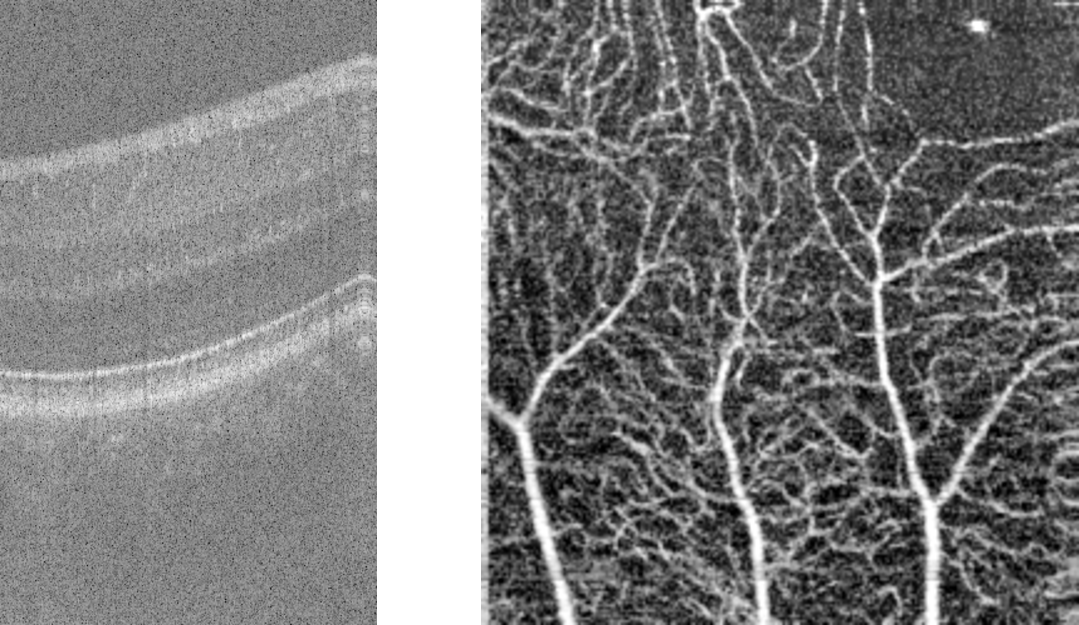
\includegraphics[width=\textwidth]{gfx/bscan_vessels}
	\caption{\textbf{Lewy obraz:} Dwuwymiarowy przekrój siatkówki oka (B-skan). Obraz został uzyskany poprzez połączenie jednowymiarowych A-skanów, które zawierają informację o strukturze tkanki w głąb siatkówki oka. \textbf{Prawy obraz:} Angiografia siatkówki oka uzyskana dzięki przetworzeniu danych z OCT.}
	\label{fig:obrazowanie_oct:bscan_vessels}
\end{figure}

% Wyjaśnia zasadę działania OCT, bez wchodzenia w duże teoretyczne detale

\section{Metoda OCT}
\label{sec:obrazowanie_oct:metoda_oct}

Jednym z najważniejszych parametrów metod tomografii w medycynie jest ich rozdzielczość. Im obrazy są bardziej dokładne, tym precyzyjniej doktorzy są w stanie zdiagnozować pacjenta. Optyczna tomografia koherencyjna przechwytuje obrazy wnętrza tkanki poprzez wykorzystanie fal świetlnych. OCT za pomocą generatora wytwarza falę świetlną, która jest skierowana na tkankę pacjenta. Następnie po odbiciu fali poprzez tkankę wiązka jest przechwycona przez detektor. Jedną z dostępnych metod, która umożliwiłaby zlokalizowanie miejsca odbicia fali byłoby zmierzenie czasu pomiędzy wygenerowaniem fali, a zarejestrowaniem jej przez detektor (mechanizm stosowany np. w ultrasonografii z wykorzystaniem fal dźwiękowych), natomiast prędkość światła (\(3\times10^8 \frac{m}{s}\)) wyklucza zastosowanie tego mechanizmu. Zjawisko, które umożliwia dokładne zlokalizowanie miejsca odbicia to \textbf{interferencja światła o niskiej spójności}.


% Wyjaśnia zasadę powstawania obrazów angiograficznych z danych OCT

\section{Angiografia OCT}
\label{sec:obrazowanie_oct:angiografia_oct}

% Opisuje zastosowania OCT

\section{Zastosowania OCT}
\label{sec:obrazowanie_oct:zastosowania_oct}















